\documentclass{report}
\usepackage[utf8]{inputenc}
\usepackage{CJKutf8}
\usepackage{amsmath}
\usepackage{tikz-qtree}
\usepackage{pgfplots}
\usepackage{hyperref}
\usepackage{graphicx}
\usepackage{cases}
\usepackage{float}
\usetikzlibrary{trees}
\title{ネットワーク設計論レポート3}
\author{27019679 グレゴリウスブライアン}
\setlength{\parindent}{0pt}

\begin{document}
\begin{CJK}{UTF8}{min}
    \maketitle


    \clearpage
    \section*{演習12問題2&3(負荷分散重み決定問題)}
    Figure 1の$e^*$で示される辺のメトリックを決定したい。同じ色の頂点対に対し$S$はソースノード、$T$はシンクノードとする。
    Figure 2とFigure 3では$e^*=\infty$と$e^*=0$の時の各ソースとシンクの最短路を表す。ただし、青の部分が両方の路が走っていて、輻輳している。$l_x^y$を
    $x=1$なら黄色対、$x=2$ならオレンジ色の頂点対の$e^*=y$の時の最短路であるとき、
    \[l_1^\infty=11,l_1^0=4\]
    \[l_2^\infty=9,l_2^0=6\]
    \[l_1=l_1^\infty-l_1^0=7\]
    \[l_2=l_2^\infty-l_2^0=3\]
    以上により$3\leq e^* \leq 7$の時、それぞれの最短路はFigure 4となり、輻輳を回避できる。
    \begin{figure}[!h]
        \centerline{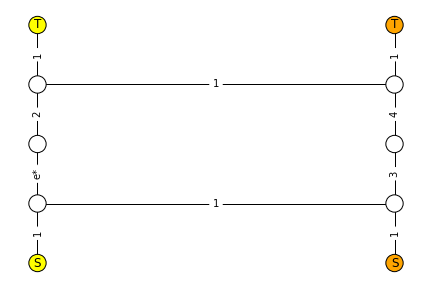
\includegraphics[width=0.8\textwidth]{data/ex12-base.png}}
        \caption{負荷分散ベースグラフ}
    \end{figure}
    \begin{figure}[!h]
        \centerline{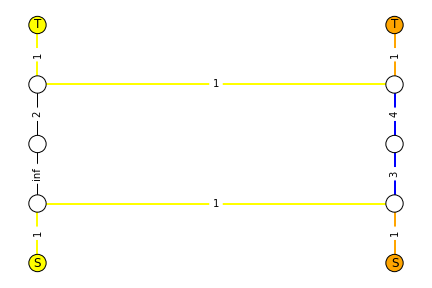
\includegraphics[width=0.8\textwidth]{data/ex12-linf.png}}
        \caption{$e^*=\infty$のとき}
    \end{figure}
    \begin{figure}[!h]
        \centerline{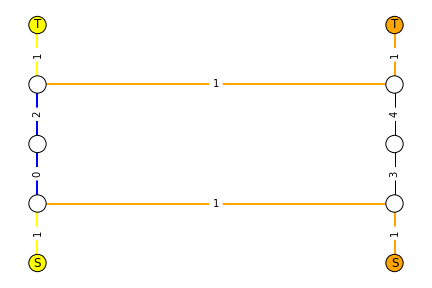
\includegraphics[width=0.8\textwidth]{data/ex12-l0.png}}
        \caption{$e^*=0$のとき}
    \end{figure}
    \begin{figure}[!h]
        \centerline{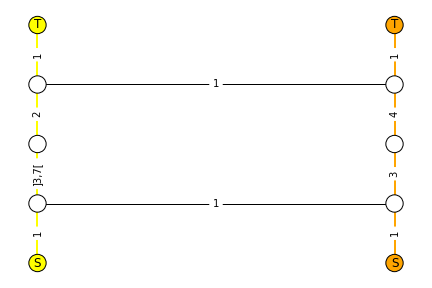
\includegraphics[width=0.8\textwidth]{data/ex12-res.png}}
        \caption{$3\leq e^* \leq 7$のとき}
    \end{figure}
    \clearpage
    \section*{演習13問題1(イプシロン劣シノプシスを用いたストリームアルゴリズム)}
    TeXの横幅(紙の幅)に上限があるため、Nが大きすぎると書ききれなくなる。
    今回扱うデータは次通りである。$N=50$で各データは独立にガウス分布 $\lceil\mathcal{N}(\mu=1000,\sigma^2=3)\rceil$ にしたがって生成される。
    $\gamma=0.3,\epsilon=0.2$と設定する。$\epsilon=0.2$のため、各バケットに入る要素数は$5$である。
    到着系列は次通りである。

    [1005, 998, 1003, 999, 1001, 1003, 997, 999, 998, 998, 1000, 1003, 1004, 1003, 1003, 999, 998, 1001, 995, 1002, 1004, 996, 1003, 1003, 1001, 998, 1000, 998, 1000, 1000, 1001, 999, 999, 997, 994, 999, 999, 1000, 1003, 999, 1007, 1000, 999, 1001, 996, 1006, 1000, 997, 1001, 1003]

    各バケット終了時の消去したものと残りの$D$は次通りである

    バケット1終了時消去:
    \[ [(1005, 1, 0), (998, 1, 0), (1003, 1, 0), (999, 1, 0), (1001, 1, 0)] \]
    バケット1終了時の$D$:
    \[ [] \]
    バケット2終了時消去:
    \[ [(1003, 1, 1), (997, 1, 1), (999, 1, 1)] \]
    バケット2終了時の$D$:
    \[ [(998, 2, 1)] \]
    バケット3終了時消去:
    \[ [(998, 2, 1), (1000, 1, 2), (1004, 1, 2)] \]
    バケット3終了時の$D$:
    \[ [(1003, 3, 2)] \]
    バケット4終了時消去:
    \[ [(999, 1, 3), (998, 1, 3), (1001, 1, 3), (995, 1, 3), (1002, 1, 3)] \]
    バケット4終了時の$D$:
    \[ [(1003, 3, 2)] \]
    バケット5終了時消去:
    \[ [(1004, 1, 4), (996, 1, 4), (1001, 1, 4)] \]
    バケット5終了時の$D$:
    \[ [(1003, 5, 2)] \]
    バケット6終了時消去:
    \[ [] \]
    バケット6終了時の$D$:
    \[ [(1003, 5, 2), (998, 2, 5), (1000, 3, 5)] \]
    バケット7終了時消去:
    \[ [(1003, 5, 2), (998, 2, 5), (1001, 1, 6), (997, 1, 6), (994, 1, 6)] \]
    バケット7終了時の$D$:
    \[ [(1000, 3, 5), (999, 2, 6)] \]
    バケット8終了時消去:
    \[ [(1003, 1, 7)] \]
    バケット8終了時の$D$:
    \[ [(1000, 4, 5), (999, 5, 6)] \]
    バケット9終了時消去:
    \[ [(1007, 1, 8), (1001, 1, 8), (996, 1, 8)] \]
    バケット9終了時の$D$:
    \[ [(1000, 5, 5), (999, 6, 6)] \]
    最終消去:
    \[ [(1006, 1, 9), (997, 1, 9), (1001, 1, 9), (1003, 1, 9)] \]
    最終の$D$:
    \[ [(1000, 6, 5), (999, 6, 6)] \]

    最終的に、$(\gamma-\epsilon)N$は$5$であり、要素1000と要素999はの$f$は両方ともこれを超えている。
    そのため、要素1000と999はこの基準において頻出と言える
    \clearpage
    \section*{添付問題(待ち行列理論)}
    \subsection*{大問1}
    \begin{enumerate}
        \item サーバーが同時に処理できるPCが1つのみとすると、窓口が1個、待ち行列の上限の長さが2であるため、
              系内人数は最大3である。到着間隔分布が指数分布に従う場合、このシステムは$M/M/1 (3)$で表記できる
        \item Figure 5が状態遷移図である。各状態に書かれている数字は系内人数である。
              \begin{figure}[!h]
                  \centerline{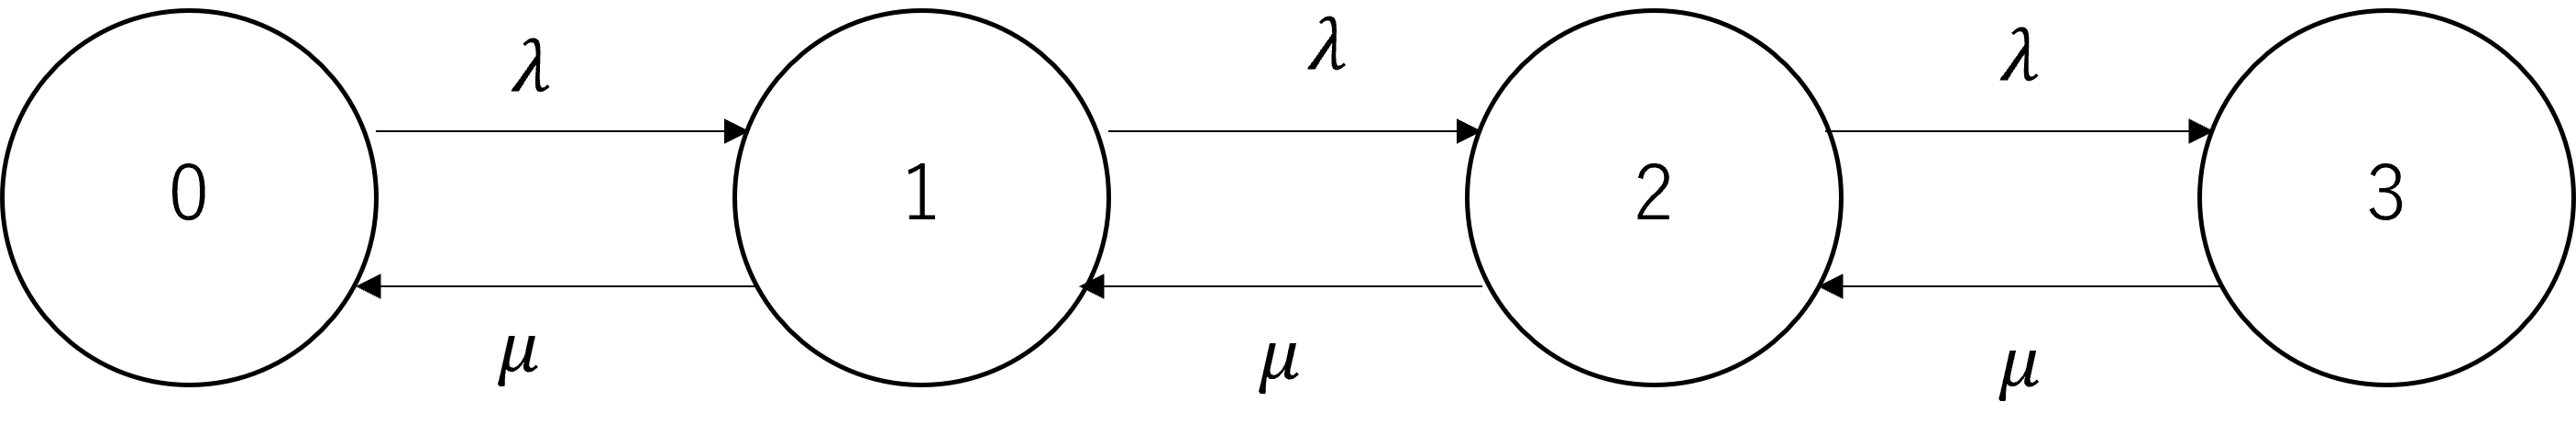
\includegraphics[width=0.8\textwidth]{data/state.png}}
                  \caption{M/M/1 (3)状態遷移図}
              \end{figure}
        \item
              \begin{numcases}{}
                  p_0\lambda=p_1\mu   \\
                  (\lambda+\mu)p_n=p_{n+1}
                  \mu+p_{n-1}\lambda&$n=1,2$\\
                  p_3\mu=p_2\lambda
              \end{numcases}
              \begin{equation}
                  \sum_{n=0}^3 p_n=1
              \end{equation}

        \item
              式$(1)$を$p_1$について解くと次になる。
              \begin{equation}
                  p_1=\frac{\lambda}{\mu}p_0
              \end{equation}
              次に$(2)$の式の左側の$p_n$を$p_1$とすると$(5)$を用いて、$p_2$について解く:
              \begin{equation}
                  \begin{aligned}[b]
                      (\lambda+\mu)p_1 & =p_{2}\mu+p_{0}\lambda      \\
                      p_{2}            & =\frac{\lambda^2}{\mu^2}p_0
                  \end{aligned}
              \end{equation}
              同様に、$(3)$と$(6)$より、
              \begin{equation}
                  p_3=\frac{\lambda^3}{\mu^3}p_0
              \end{equation}
              式$(3)$を変形し、既知の関係式を代入すると
              \begin{equation}
                  \begin{aligned}[b]
                      \sum_{n=0}^\infty p_n & =1                                                \\                                                                                                \\
                      p_0                   & =\frac{1}{1+\sum_{n=1}^3 \frac{\lambda^n}{\mu^n}}
                  \end{aligned}
              \end{equation}
              $\rho=\lambda/\mu$を用いると
              \begin{equation}
                  p_0=\frac{1}{1+\sum_{n=1}^3 \rho^n}
              \end{equation}
              \begin{equation}
                  p_1=\frac{\rho}{1+\sum_{n=1}^3 \rho^n}
              \end{equation}
              \begin{equation}
                  p_2=\frac{\rho^2}{1+\sum_{n=1}^3 \rho^n}
              \end{equation}
              \begin{equation}
                  p_3=\frac{\rho^3}{1+\sum_{n=1}^3 \rho^n}
              \end{equation}
        \item
              \begin{equation}
                  \lambda=45/3600=1/80
              \end{equation}
              \begin{equation}
                  \mu=1/75
              \end{equation}
              \begin{equation}
                  \rho=75/80
              \end{equation}

        \item 呼損率は系内人数が最大である確率である。式$(8)$を用いて$p_0\approx0.275$であることがわかるので呼損率$p_3\approx 0.226$である。
        \item 呼損率が1%以下に抑えたいなら、系内人数を99人以上にする必要がある。つまり待ち行列長を98以上にする必要がある。
              なぜなら、アクセス頻度増加により、$\mu=\lambda$になり$\rho=1$になる。このとき、式(10)から(13)により、すべての状態の確率が$p_0$と等しくなる。状態の数$N$は系内人数$K$+1である。
              各状態の確率は等しいかつすべての状態確率の和が1のため、各状態の確率は$1/N$である。呼損率は系内人数が最大の状態であるため、呼損率を1%以下にするために、$1/N\leq0.01$を満たす必要がある。$N$について解けば$N\geq100$がわかる。
              よって、$N=100$が最低限の状態の数である。$N=100$のときの系内人数は$K=99$である。このとき、待ち行列長が$98$である。
    \end{enumerate}
    \subsection*{大問2}
    \begin{enumerate}
        \item $M/M/2(2)$
        \item Figure 6
              \begin{figure}[!h]
                  \centerline{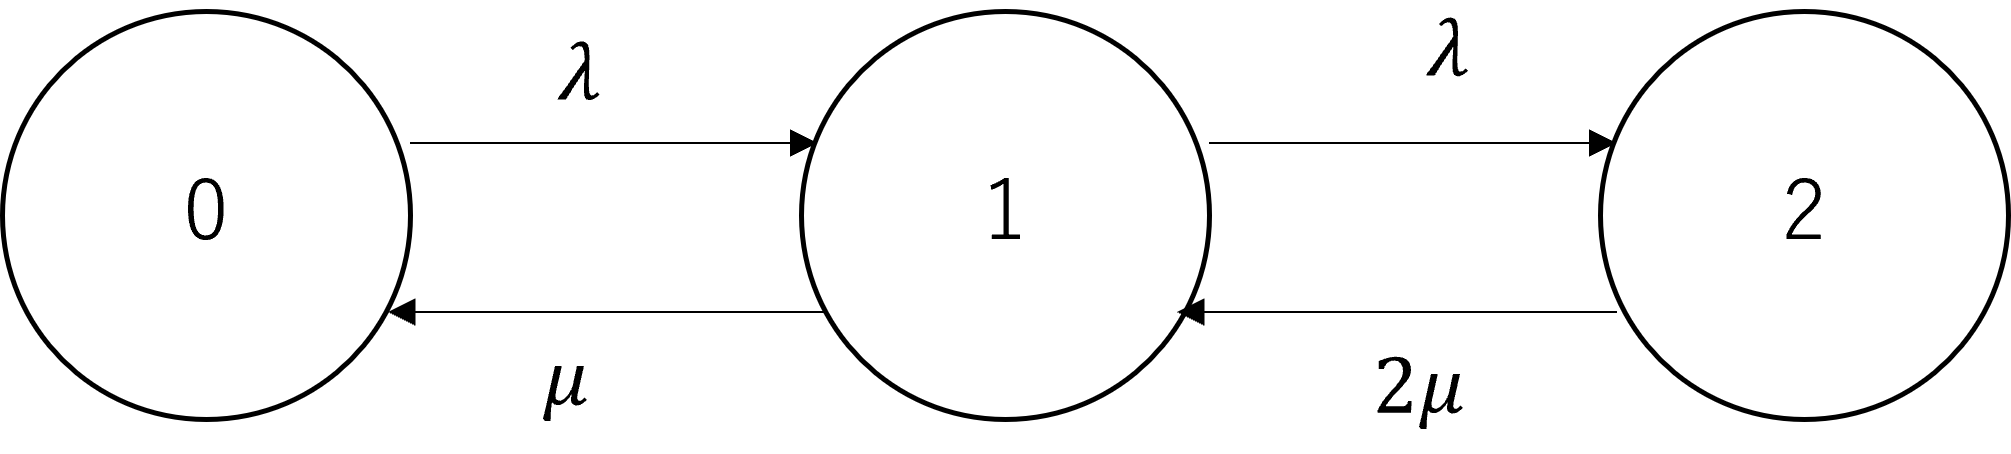
\includegraphics[width=0.8\textwidth]{data/state2.png}}
                  \caption{M/M/2(2)状態遷移図}
              \end{figure}
        \item
              \begin{numcases}{}
                  p_0\lambda=p_1\mu   \\
                  \lambda p_0 +2\mu p_2 = (\mu+\lambda)p_1\\
                  2\mu p_2=\lambda p_1
              \end{numcases}
              \begin{equation}
                  \sum_{n=0}^2 p_n=1
              \end{equation}
        \item $\rho=\lambda/\mu$を用いて(16)より
              \begin{equation}
                  p_1=\rho p_0
              \end{equation}
              (18),(19)より、
              \begin{equation}
                  \begin{aligned}[b]
                      2\mu p_2=\lambda \rho p_0 \\
                      p_2=\frac{\rho^2p_0}{2}
                  \end{aligned}
              \end{equation}
              (19)(20)(21)より、
              \begin{equation}
                  \begin{aligned}[b]
                      p_0(1+\rho+\frac{\rho^2}{2})=1 \\
                      p_0=\frac{2}{2+2\rho+\rho^2}
                  \end{aligned}
              \end{equation}
              \begin{equation}
                  p_1=\frac{2\rho}{2+2\rho+\rho^2}
              \end{equation}
              \begin{equation}
                  p_2=\frac{\rho^2}{2+2\rho+\rho^2}
              \end{equation}
        \item
              \begin{equation}
                  \lambda=\frac{10}{60}=\frac{1}{6}
              \end{equation}
              \begin{equation}
                  \mu=\frac{1}{10}
              \end{equation}
              \begin{equation}
                  \rho=\frac{10}{6}
              \end{equation}
        \item 呼損率
              \begin{equation}
                  \begin{aligned}[b]
                      p_2=\frac{\rho^2}{2+2\rho+\rho^2} \\
                      p_2\approx0.342
                  \end{aligned}
              \end{equation}
    \end{enumerate}

    \clearpage
    \section*{添付問題(ネットワーク構造設計)}
    \subsection*{大問1}
    \begin{enumerate}
        \item $k$辺連結成分とは$V$の直和分割$\{V_1,V_2,\dots,V_p\}$で、各$V_i (1\leq i \leq p)$に対して次を満たす
              \begin{enumerate}
                  \item $x,y\in V_i (x\neq y)$の任意の$x$と$y$に対して、局所辺連結度は$k$以上である
                  \item $x\in V_i, y\in V_j$ $(i\neq j)$の任意の$x$と$y$に対して、局所辺連結度は$k$未満である
              \end{enumerate}
        \item Figure 7。同じ色同氏は同じグループにある。
              \begin{figure}[!h]
                  \centerline{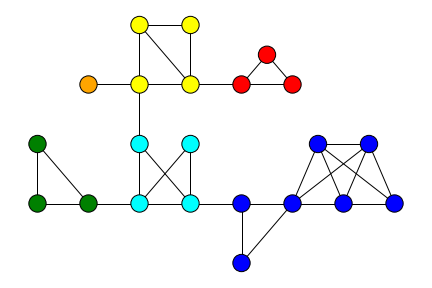
\includegraphics[width=0.8\textwidth]{data/k-connect.png}}
                  \caption{$G$の2辺連結成分分解}
              \end{figure}
        \item Figure 7のオレンジ、赤、緑、青成分
        \item どの一本のリンクが切れても接続可能の配置は2-NA辺連結になるように領域を決めると等しい。そうするためには、(3.)で答えた不足成分内のそれぞれ1頂点を領域にすればいい。
    \end{enumerate}
    \subsection*{大問2}
    \begin{enumerate}
        \item 原則任意の頂点対の局所辺連結度が$k$以上であるが、元々のグラフで局所辺連結度が$k$未満である頂点対にたいし、現状維持する。
        \item
              \begin{enumerate}
                  \item Figure 8
                        \begin{figure}[!h]
                            \centerline{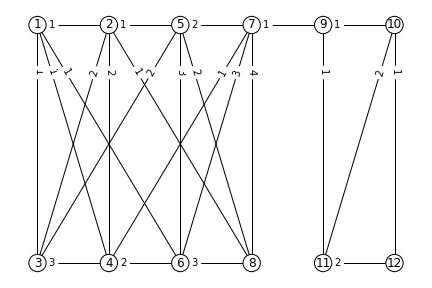
\includegraphics[width=0.8\textwidth]{data/MA.png}}
                            \caption{$G$の2辺連結成分分解}
                        \end{figure}
                  \item Figure 9
                        \begin{figure}[!h]
                            \centerline{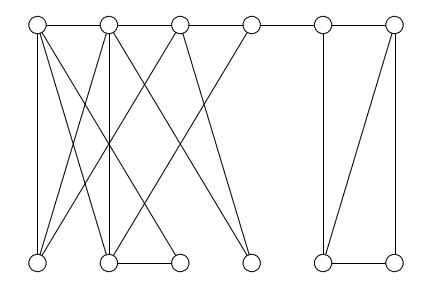
\includegraphics[width=0.8\textwidth]{data/k-save.png}}
                            \caption{$G_2$($G$の2辺連結性保存)}
                        \end{figure}
              \end{enumerate}

        \item $G_k=F_1\cup F_2 \cup \dots \cup F_k$で求められ、各$F_i (1\leq i \leq k)$は森であるため、
        $F_i$の辺の数は$|V|-1$以下である。$G_k$はそういう$F_i$を$k$をユニオンしたグラフであるため$G_k$の変数は$k(|V|-1)$である。
        \item $k$辺連結性を保存する最小変数の全域部分グラフは最低でも$k|V|/2$個の辺の持つ。この2倍は$k|V|$であり、
        3.からこのアルゴリズムは変数$k(|V|-1)$個以下の辺を持つ全域部分グラフを生成する。$k(|V|-1)<k|V|$であるため、
        このアルゴリズムは最適解の高々2倍近似であることがわかる。
    \end{enumerate}
\end{CJK}



\end{document}
